\section{Discussion}

The estimator is not a pure cumulant-propagation or covariance-propagation method \citep{wright2024analytic, wu2026estimating}. Instead, it combines analytical approximations with antithetic Sobol sampling. Its primary mechanistic contribution is using structural information about the MLP to sample more strategically: the diagonal Gaussian pass first predicts which neurons are dead, kink, and on; the pilot samples refine uncertain classifications; and the resulting activation structure determines both which neurons are sampled and how the sampled matrix products are evaluated. We hope our methods can serve as a sampling baseline for more sophisticated white-box estimators that exploit the same mechanistic structure.

The main limitation is that the estimator does not yet eliminate sampling variance at the kink paths. Better mechanistic progress would replace more of the sampled active path with a controlled low-order distributional approximation, or identify which cross-neuron dependencies matter enough to track. Recent analytic covariance-propagation work gives one example of a more ambitious second-order direction \citep{wright2024analytic}. On the compute side, the packed prefix removes the cold-band zeros, but roughly a third of the zeros are scattered through the hot block, whose rows are dense enough that per-element gather pricing makes them too expensive to skip. The hot block is also numerically low-rank: about eight directions carry ${\sim}99\%$ of its second-moment energy. We could not turn that into a saving, however. Truncating the hot block to low rank perturbs every sample in a correlated way, ReLU turns that perturbation into bias on the scored means, and the measured bias was orders of magnitude above what the score can absorb. So there is clearly structure left on the table; what is missing is a way to use it without giving up exactness.

A useful stress test is to ask whether the same hard regimes would arise under smooth activations. \Cref{fig:activation-function-regimes,fig:activation-function-design-matrices,fig:activation-function-covariance} repeats the diagnostic on matched random MLPs with ReLU, GELU \citep{hendrycks2016gelu}, and SiLU \citep{elfwing2018silu}, using the same ReLU-He weight scaling. The result is not activation-agnostic. ReLU creates literal always-off and always-on regions, which justify exact dead pruning and linear folds. GELU and SiLU have no hard zero or identity region, so the same visualization should be read as scale and curvature rather than dead/on classification. In particular, the SiLU panels shrink strongly toward near-zero activations under this ReLU-tuned initialization; this is an activation-scale collapse, not a dying-ReLU phenomenon. The broader lesson is still mechanistic: inspect the activation distribution and sample matrix first, then choose the computation that matches that network's behavior.

\begin{figure}[p]
	\centering
	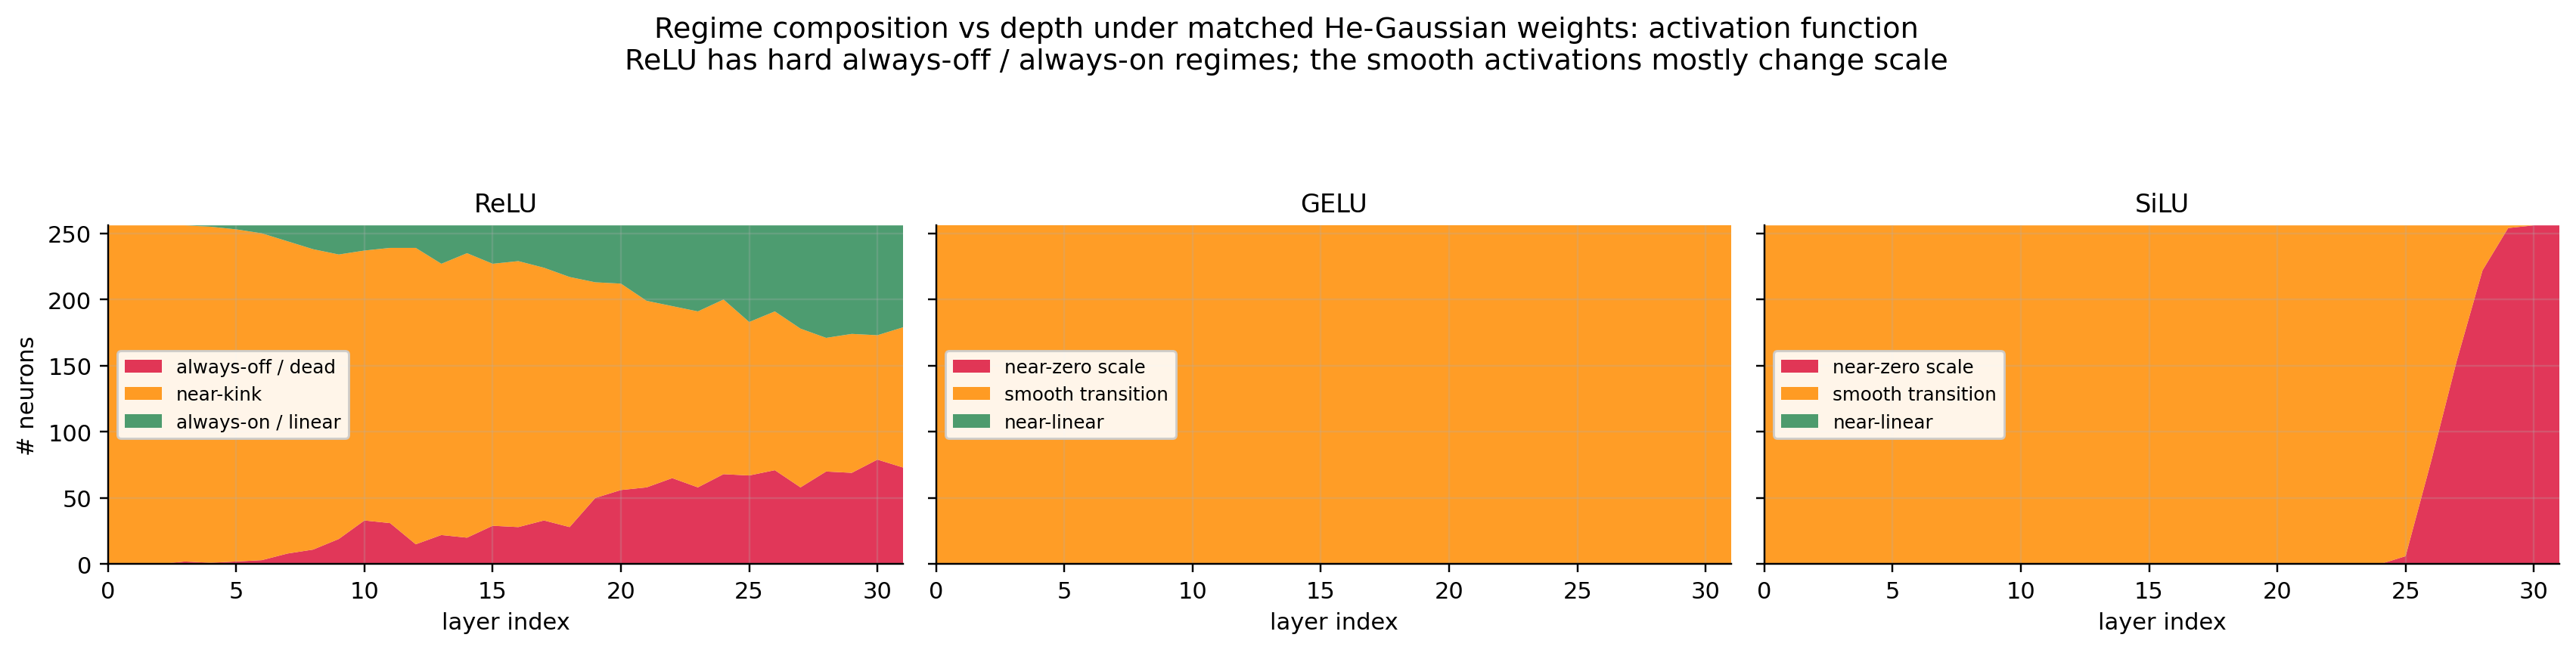
\includegraphics[width=\linewidth]{figures/activation_function_regime_comparison.png}
	\caption{Matched random MLPs with ReLU, GELU, and SiLU under the same ReLU-He weight scaling. ReLU develops hard always-off, near-kink, and always-on populations. Smooth activations do not have literal dead/on regimes; the GELU and SiLU panels instead show how much of the network is in a smooth transition or near-zero-scale region under this initialization.}
	\label{fig:activation-function-regimes}
\end{figure}

\begin{figure}[p]
	\centering
	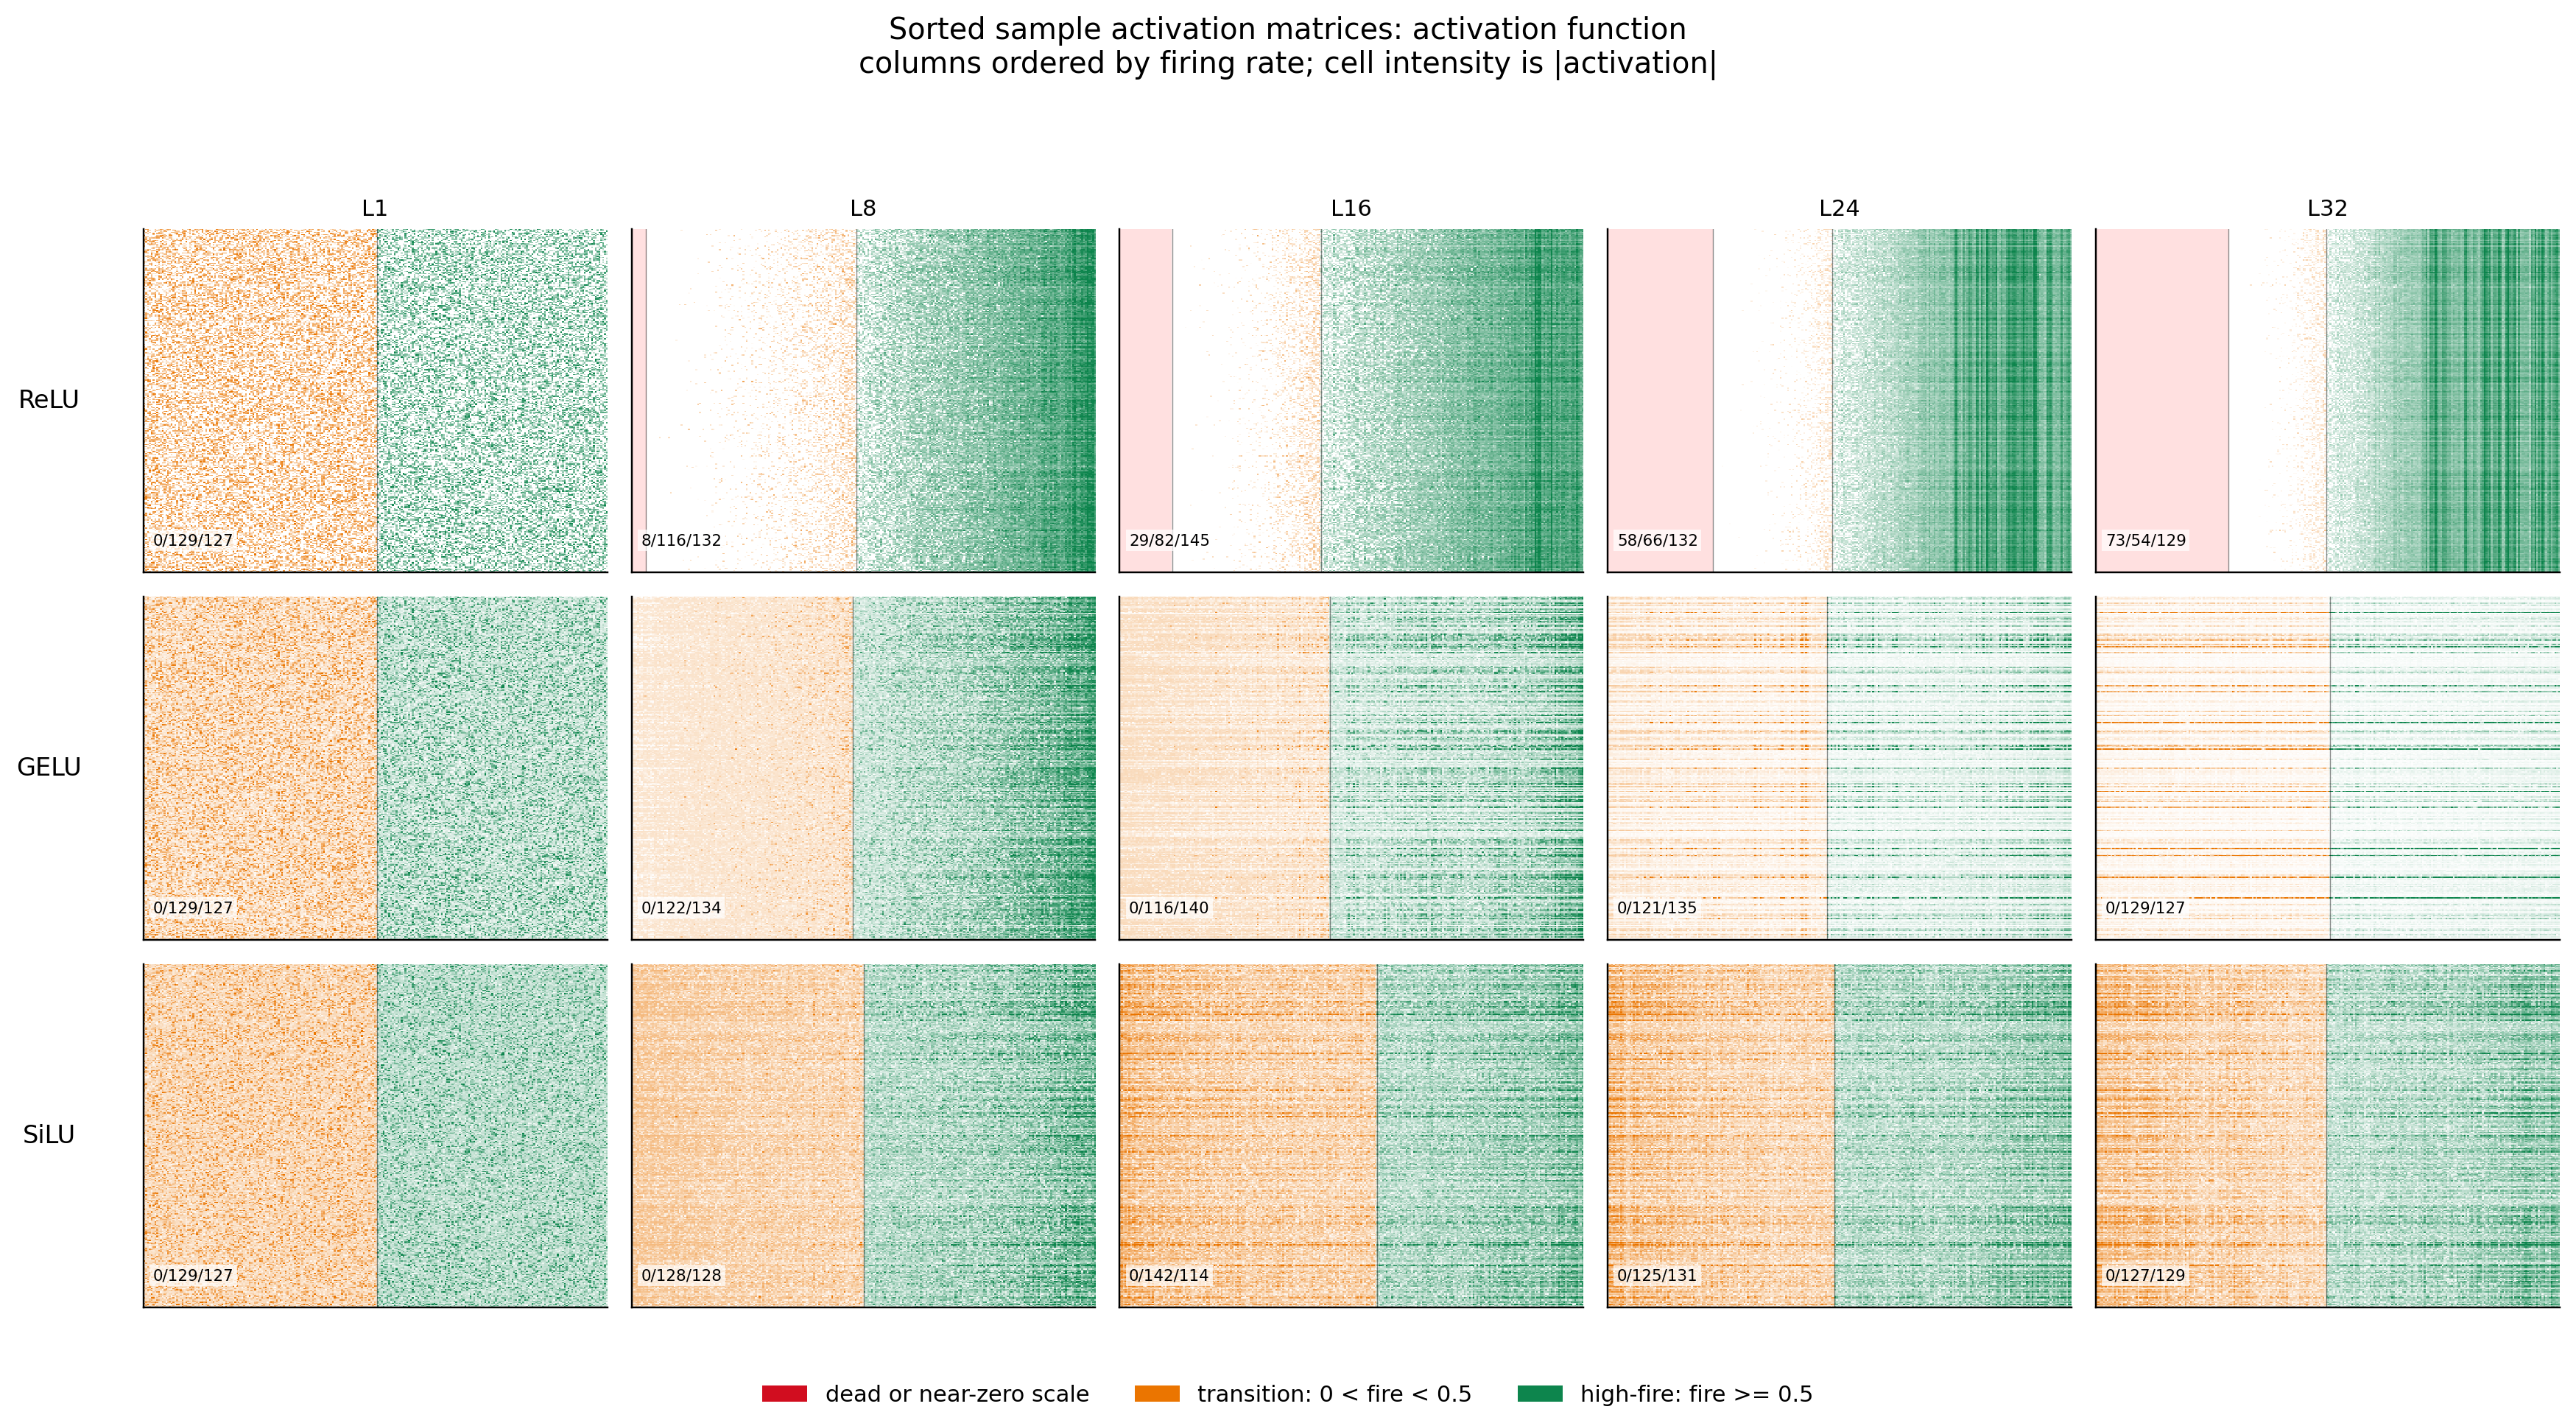
\includegraphics[width=\linewidth]{figures/activation_function_design_matrix_comparison.png}
	\caption{Sorted sample activation matrices for the same matched networks. Columns are ordered by firing rate and intensities show absolute activation magnitude. The ReLU row has a literal blank dead block, a transition block, and a dense high-fire block. The smooth activations retain transition-like columns; the SiLU final layer appears blank because the activation scale has collapsed under this ReLU-tuned initialization.}
	\label{fig:activation-function-design-matrices}
\end{figure}

\begin{figure}[p]
	\centering
	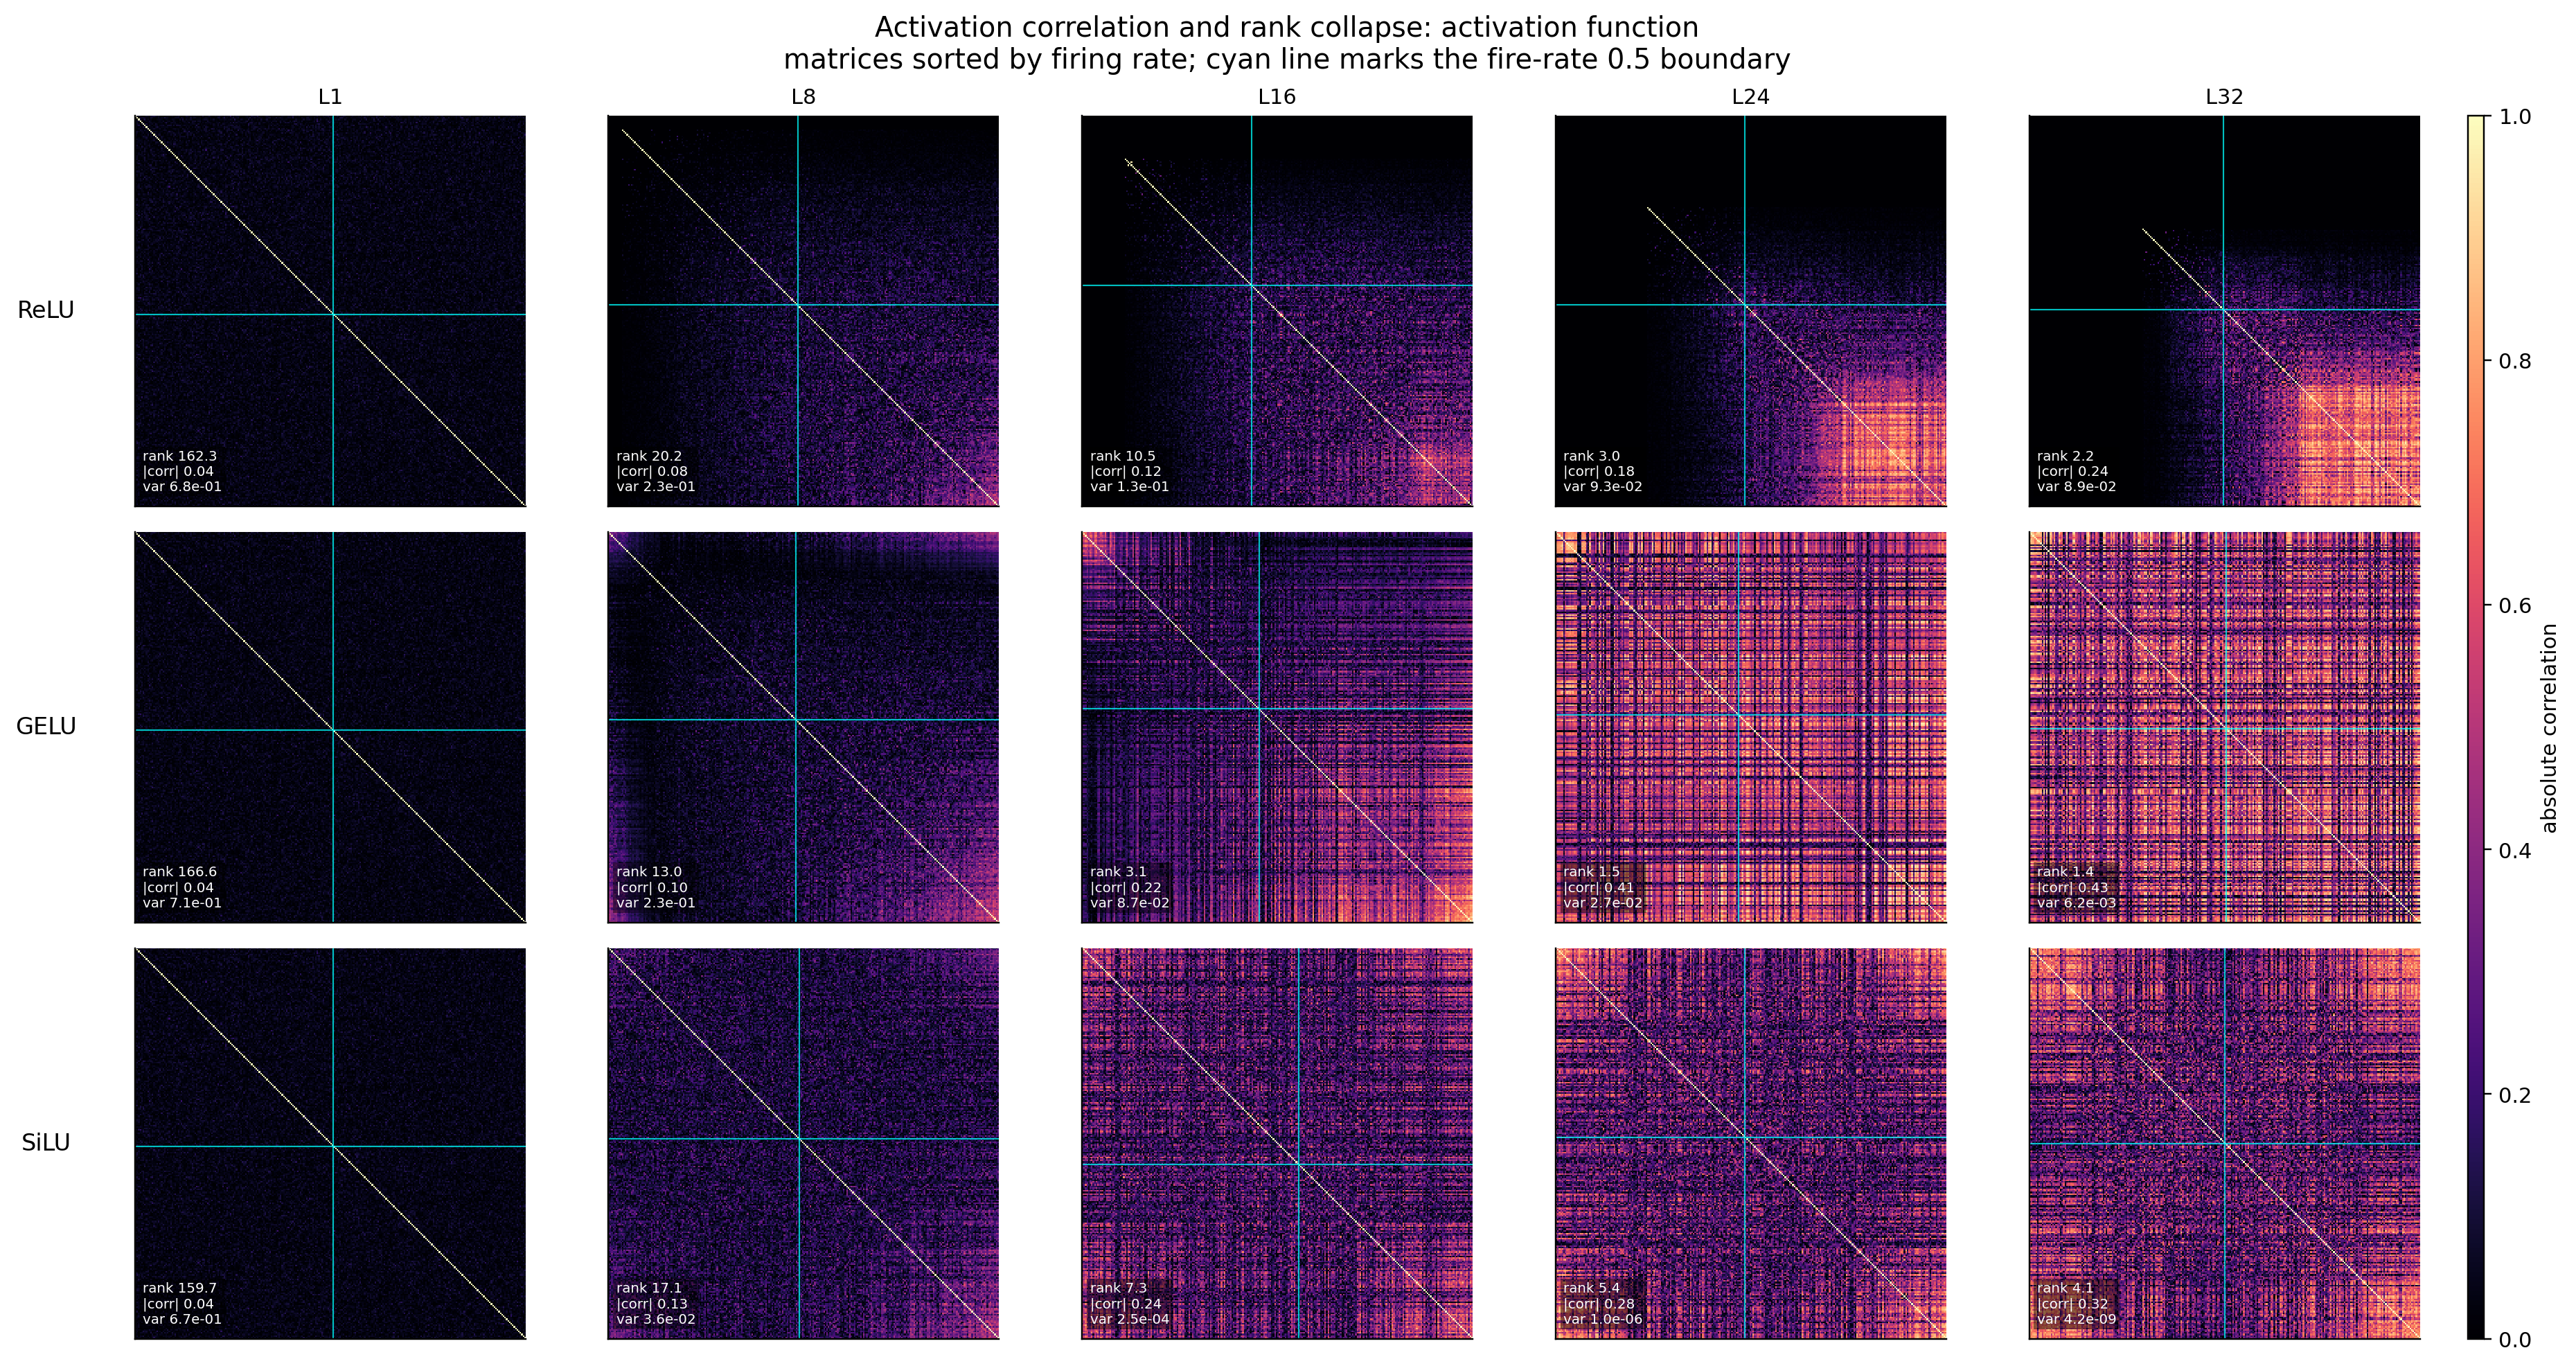
\includegraphics[width=\linewidth]{figures/activation_function_covariance_comparison.png}
	\caption{Activation covariance and rank-collapse comparison for the matched activation functions. The colorbar is shared across all panels and placed outside the heatmaps. ReLU keeps a hard firing-rate boundary with a concentrated late correlated core; GELU and SiLU also show rank collapse, but without the exact ReLU dead/on identities used by the submitted estimator.}
	\label{fig:activation-function-covariance}
\end{figure}

For the purposes of the challenge, the result shows that white-box structure can substantially improve the compute-accuracy tradeoff over plain sampling. For the broader mechanistic-estimation agenda, the lesson is narrower but encouraging: even a simple Gaussian regime classifier can turn a random MLP into a smaller estimation problem whose remaining uncertainty is localized and measurable.